In this part of the document we'll talk about the Hennessy-Milner
logic over CCS processes. We approach the logic in two steps: the
former without recursion, where we'll use the logic to show the
non-bisimilarity of toy processes; the latter including recursion
operators, where we'll build a simple model involving a car and a
train, aiming to verify some safety and liveness properties.

\section{$\mu$-calculus definition}
Following \cite{MuScSt1999}, $\mu$-calculus formulae are constructed
according to the following grammar:
\begin{displaymath}
  \phi := tt \mid ff \mid \phi_1 \wedge \phi_2 \mid \phi_1 \vee \phi_2 \mid
  \langle a \rangle \phi \mid [a]\phi \mid X \mid \mu X.\phi
  \mid \nu X.\phi
\end{displaymath}
where $a \in Act$, $X \in Var$, $tt$ means \emph{true} and $ff$ means
\emph{false}. The fixpoint operators $\mu X.\phi, \nu X.\phi$ bind
free occurrences of variable $X \in Var$.

Formulae that can be composed using the syntax above are interpreted
over \emph{Labeled Transition Systems}. Given an \emph{Labeled
  Transition Systems} $T = (S, Act, \rightarrow)$, we interpret a
\emph{closed} formula $\phi$ as the subset of states whose make $\phi$
true while we interpret an \emph{open} formula using a function (also
called \emph{environment}) $\rho$ such that $\rho: Var \rightarrow
2^S$. Roughly speaking, $\rho(X)$ interprets a free variable $X$
contained in a formula $\phi$ by a subset of $S$, representing an
assumption about the set of states satisfying the subformula $X$.

Let $T = (S, Act, \rightarrow)$ be a \emph{Labeled Transition
  Systems}, $\phi$ a formula and $\rho$ an environment, we define the
set $\mathcal{M}_T(\phi, \rho) \subseteq S$ satisfying $\phi$ is
defined inductively as follows:
\begin{displaymath}
  \begin{split}
    \mathcal{M}_T(tt, \rho) &= S \\
    \mathcal{M}_T(ff, \rho) &= \emptyset \\
    \mathcal{M}_T(\phi_1 \wedge \phi_2, \rho) &=
    \mathcal{M}_T(\phi_1, \rho) \cap     \mathcal{M}_T(\phi_2, \rho)\\
    \mathcal{M}_T(\phi_1 \vee \phi_2, \rho) &=
    \mathcal{M}_T(\phi_1, \rho) \cup     \mathcal{M}_T(\phi_2, \rho)\\
    \mathcal{M}_T([a]\phi, \rho) &= \{ s\in S: \forall s^{\prime}: s
    \xrightarrow{a} s^{\prime} \rightarrow s^{\prime} \in
    \mathcal{M}_T(\phi, \rho)\} \\
    \mathcal{M}_T(\langle a \rangle \phi, \rho) &= \{ s\in S: \exists
    s^{\prime}: s \xrightarrow{a} s^{\prime} \wedge s^{\prime} \in
    \mathcal{M}_T(\phi, \rho)\} \\
    \mathcal{M}_T(X, \rho) &= \rho(X) \\
    \mathcal{M}_T(\mu X.\phi, \rho) &= fix_{\mu}F_{\phi, \rho, X} \\
    \mathcal{M}_T(\nu X.\phi, \rho) &= fix_{\nu}F_{\phi, \rho, X} \\
  \end{split}
\end{displaymath}
where $fix_{\mu}F_{\phi, \rho, X}, fix_{\mu}F_{\phi, \rho, X}$ mean
the least and greater fixed points of the function $F_{\phi, \rho, X}:
2^S \rightarrow 2^S$, which is defined as:
\begin{displaymath}
  F_{\phi, \rho, X}(x) = \mathcal{M}_T(\phi, \rho_{X, x, \rho}^{\prime})
\end{displaymath}
where $\rho_{X, x, \rho}^{\prime}: Var \rightarrow 2^S$ is defined as:
\begin{displaymath}
  \begin{split}
    \rho_{X, x, \rho}^{\prime}(X) &= x \\
    \rho_{X, x, \rho}^{\prime}(Y) &= \rho(Y) \quad \text{if } X\not=Y\\
  \end{split}
\end{displaymath}




\begin{verbatim}
Process s: RecX(a?.b?.RecY((b?.Y + a?.X)))
Process t: RecX(a?.RecY((b?.Y + b?.a?.X)))
Process v: RecX(a?.(b?.b?.RecY((b?.Y + a?.X)) + b?.RecY((b?.Y + a?.X))))

s isn't  bisimilar to t due to formula f= [a][b]<a>tt
s satisfy f: true
t satisfy f: false


s isn't  bisimilar to v due to formula f= [a]<b>[a]ff
s satisfy f: false
v satisfy f: true


t isn't  bisimilar to v due to formula f= [a]<b>[b]ff
t satisfy f: true
v satisfy f: false
\end{verbatim}
The processes under study are taken from \cite{1324845} and are
reported in \autoref{fig:not-bisimilar-processes}.
\begin{figure}[htb]
  \centering
  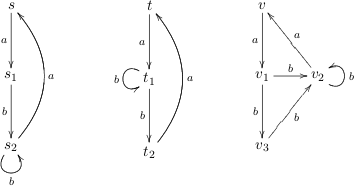
\includegraphics{qualitative-project/not-bisimilar-processes.png}
  \caption{Three not bisimilar processes}
  \label{fig:not-bisimilar-processes}
\end{figure}
